\documentclass[preprint,12pt]{elsarticle}
\usepackage{amssymb}
\usepackage{amsmath}
\usepackage{booktabs}
\usepackage{graphicx}
\usepackage{float}
\usepackage{tikz}
\usetikzlibrary{arrows.meta,positioning}
\usepackage{url}
\journal{Knowledge-Based Systems}

%% ---------- Notation ----------
% EU / AU measures: superscript = variant (h: hard split with 5 neighbours, s: soft split with 15 neighbours
% and plain votes, sb: soft split with 15 neighbours and class-balanced votes)
\newcommand{\EUmin}[1]{\mathrm{EU}^{\mathrm{#1}}_{\min}}
\newcommand{\EUdif}[1]{\mathrm{EU}^{\mathrm{#1}}_{\Delta}}
\newcommand{\AUbal}[1]{\mathrm{AU}^{\mathrm{#1}}}
\newcommand{\IR}{\mathrm{IR}}
\newcommand{\UNS}{\mathrm{UNS}}
\newcommand{\RO}{\mathrm{RO}}
\newcommand{\Nbal}{\mathrm{N3}_{\mathrm{bal}}}
\newcommand{\todo}[1]{\textbf{[TODO: #1]}}

\sloppy
\begin{document}
\begin{frontmatter}

\title{Measuring class imbalance complexity through classifier uncertainty: when does oversampling pay off?}

\author[omu]{Fatih Sa\u{g}lam\corref{cor1}}
\ead{fatih.saglam@omu.edu.tr}
\cortext[cor1]{Corresponding author. ORCID: 0000-0002-2084-2008}
\affiliation[omu]{organization={Department of Statistics, Faculty of Science, Ondokuz May{\i}s University},
            postcode={55100},
            city={Samsun},
            country={T\"urkiye}}

\begin{abstract}
Class imbalance hurts some datasets and leaves others untouched, and the imbalance ratio (IR) does not tell them apart. The harm also depends on the classifier, but the complexity measures in the literature are computed from the data alone and give the same value for every classifier. We propose complexity measures for class imbalance that depend on the classifier. They use out-of-bag predictions from bootstrap ensembles and split each case's error into an aleatoric part (label noise and overlap) and an epistemic part (disagreement between the model and the local, class-balanced evidence). In a simulation with five data families, six imbalance ratios and seven classifiers, the epistemic measure built on a class-balanced 15-neighbour vote correlates 0.87 to 0.89 with the G-mean lost to imbalance, stays between 0.80 and 0.95 for every classifier, and adds information beyond IR. Variants with plain votes or a hard 5-neighbour split do not. On 30 real datasets from the UCI and KEEL repositories it correlates 0.75 with the G-mean gain from SMOTE, and the epistemic difference variant keeps a partial correlation of 0.58 after controlling for baseline performance. A threshold of about 0.17 on the epistemic measure tells whether SMOTE pays off for the G-mean, with a cross-validated balanced accuracy of 0.82 against 0.69 for IR. The measures grow with IR on separable data, and the aleatoric measures are weaker; we report both limits.
\end{abstract}

\begin{highlights}
\item Classifier-aware epistemic and aleatoric complexity measures for class imbalance
\item A class-balanced neighbour vote is the key ingredient of the epistemic measure
\item Adds information beyond the imbalance ratio across seven classifiers
\item Correlates with the gain from oversampling on 30 real datasets
\item A threshold on it tells when oversampling is worth doing
\end{highlights}

\begin{keyword}
class imbalance \sep data complexity \sep epistemic uncertainty \sep aleatoric uncertainty \sep oversampling
\end{keyword}

\end{frontmatter}

\section{Introduction}\label{sec:intro}
A binary classifier trained on imbalanced data usually predicts the minority class worse than the majority class, and a large part of the machine learning literature on imbalance is about repairing this with resampling, cost-sensitive learning or ensembles \cite{He2009,Fernandez2018}. Before choosing a remedy, a practitioner would like to know how much the imbalance in the data at hand actually costs. Three facts make this question hard.

\textbf{The harm of imbalance is not explained by the imbalance ratio.} The imbalance ratio ($\IR$, the number of majority cases divided by the number of minority cases) is the usual summary, but it ignores the geometry of the data. Two datasets with the same $\IR$ can behave very differently: if the classes are well separated, a classifier can learn the boundary from few minority cases and the imbalance does little damage, while the same $\IR$ in a region where the classes overlap, or where the minority is split into small disjuncts, can ruin minority performance \cite{Japkowicz2002,Prati2004,Lopez2013,Santos2022}.

\textbf{Resampling does not always help.} Oversampling methods such as SMOTE \cite{Chawla2002} are applied routinely, but their benefit varies from dataset to dataset and is sometimes negative. A measure that indicates when rebalancing is worth doing would be more useful than a measure that only describes how imbalanced the data are.

\textbf{The harm depends on the classifier.} A flexible classifier such as a random forest and a linear classifier such as logistic regression lose different amounts on the same imbalanced dataset, and so do the gains from resampling. Data complexity measures \cite{Ho2002,Lorena2019}, including those designed for imbalanced data \cite{Barella2021,Napierala2016}, are computed from the feature matrix and the labels only. They return the same value whatever classifier will be used. To our knowledge there is no classifier-based complexity measure for class imbalance.

This paper proposes such a measure. The idea is to ask the classifier itself where it is wrong and to separate two kinds of errors. Some errors are unavoidable because the classes are mixed in the neighbourhood of the case (aleatoric uncertainty). Others occur although the neighbourhood is clear, because the model has too little information or too little flexibility there (epistemic uncertainty). Imbalance makes the second kind worse, and it is the kind that more minority information, from data collection or from resampling, can remove. We estimate both parts from the out-of-bag predictions of a bootstrap ensemble of the classifier of interest, so that the measure is defined for any classifier and for the hyperparameters the user will actually use.

The contributions of this paper are:
\begin{enumerate}
\item Epistemic and aleatoric complexity measures for class imbalance that depend on the classifier, with a hard 5-neighbour and a soft 15-neighbour version, and a class-balanced neighbour vote that proves to be the key ingredient.
\item A simulation study with five data families, six imbalance ratios and seven classifiers, comparing the measures with $\IR$ and with measures from the literature, for each classifier separately.
\item A study on 30 real datasets relating the measures to the gain from oversampling, for each classifier separately.
\item A preliminary guide that tells, from the value of the measure, whether oversampling is worth doing for a given classifier and metric, with a version that also uses the aleatoric measure.
\item An account of the limits of the measures: their growth with $\IR$ on separable data and the weaker results of the aleatoric measures.
\end{enumerate}

Section~\ref{sec:related} reviews related work. Section~\ref{sec:unc} explains aleatoric and epistemic uncertainty and how they relate to imbalance. Section~\ref{sec:method} defines the measures. Section~\ref{sec:design} describes the simulation and the real-data experiments, and Section~\ref{sec:results} reports their results. Section~\ref{sec:disc} discusses limitations and Section~\ref{sec:concl} concludes.

%% =====================================================================
\section{Related work}\label{sec:related}
\subsection{Class imbalance and its sources of difficulty}
Learning from imbalanced data is surveyed in~\cite{He2009,Fernandez2018}. Early systematic studies showed that imbalance alone is not always harmful and that its effect grows with the complexity of the concept and with a small training set~\cite{Japkowicz2002}. Later work identified class overlap~\cite{Prati2004,Vuttipittayamongkol2021}, small disjuncts~\cite{Jo2004}, and borderline, rare and noisy minority cases~\cite{Napierala2016} as main sources of the damage, and studied them jointly~\cite{Lopez2013,Santos2022}. Remedies include resampling, cost-sensitive learning and ensembles. Random oversampling and SMOTE~\cite{Chawla2002} are the standard resampling methods, and the benefit of balancing varies between datasets and classifiers~\cite{Batista2004}. Our simulation families (separable, overlapping, disjunct and noisy) follow this view of the sources of difficulty.

\subsection{Data complexity measures}
Data complexity measures describe how difficult a classification problem is from the data alone. They were introduced by Ho and Basu~\cite{Ho2002} and are surveyed by Lorena et al.~\cite{Lorena2019}, whose categories we follow. We list the measures that we use as competitors, with a sentence on what each one does.

\textbf{Feature-based measures} look at the overlap of the classes along individual features. F1 is the largest Fisher discriminant ratio over the features, and F1v is the same ratio along the best linear direction. F2 is the volume of the region in which the class-conditional ranges of the features overlap. F3 is the share of cases that lie in the overlap region of the best single feature. F4 is the share of cases that remain in overlap after the features have been used in turn to separate cases (collective feature efficiency)~\cite{Ho2002,Lorena2019}.

\textbf{Neighbourhood-based measures} look at the local structure of the classes. N1 is the share of cases that are joined to a case of the other class in a minimum spanning tree. N2 is the ratio of the mean within-class to the mean between-class nearest-neighbour distance. N3 is the leave-one-out error of the 1-nearest-neighbour classifier. N4 is the error of the 1-nearest-neighbour classifier on synthetic points interpolated between cases of the same class. LSC, the local set cardinality, counts for each case the cases that are closer to it than its nearest case of the other class~\cite{Ho2002,Lorena2019,Leyva2015}.

\textbf{Class-balance measures} describe the class sizes. C1 is the entropy of the class proportions and C2 is derived from the imbalance ratio~\cite{Lorena2019}. The imbalance ratio $\IR$ is the ratio of the class sizes, and the imbalance degree measures the distance of the class proportions from the balanced distribution~\cite{Ortigosa2017}. For two classes all of these are monotone functions of $\IR$ and rank datasets in the same way, so we report $\IR$ only.

\textbf{Imbalance-oriented measures} describe the minority class. Napierala and Stefanowski~\cite{Napierala2016} label each minority case as safe, borderline, rare or outlier according to the number of minority cases among its nearest neighbours; the shares of unsafe, and of rare and outlier, minority cases are used as measures of minority difficulty. Barella et al.~\cite{Barella2021} adapted classical complexity measures to imbalanced data, and showed that the change in complexity after resampling correlates with the change in performance.

\textbf{Using complexity measures to anticipate the effect of a treatment.} Complexity measures have been used to predict when noise filtering helps a nearest-neighbour classifier~\cite{Saez2013} and to delimit the domains of competence of classifiers~\cite{Luengo2015}. Instance hardness~\cite{Smith2014} is defined through the misclassification of a set of learning algorithms, but it describes single cases, not the imbalance of a dataset. The dataset-level measures above are computed from the features and labels alone, so they return the same value for every classifier.

\subsection{Uncertainty in machine learning}
The split of predictive uncertainty into an aleatoric and an epistemic part is well established~\cite{DerKiureghian2009,Hullermeier2021}. For classification, Senge et al.~\cite{Senge2014} learn classifiers that report both parts, and for deep networks both parts are modelled and estimated with ensembles or with Bayesian approximations~\cite{Kendall2017,Lakshminarayanan2017}. We use the split to describe how a dataset is difficult for a given classifier, not to quantify the uncertainty of a prediction.

\textbf{Uncertainty in oversampling.} Several oversampling methods use uncertainty to decide where to generate cases. Active-learning approaches select informative cases, typically those the current model is least sure about. Ertekin~\cite{Ertekin2013} creates minority cases during training in this way, and Attenberg and Ertekin~\cite{Attenberg2013} review active learning for imbalanced data. Grina et al.~\cite{Grina2021} use evidence theory to model uncertainty and to treat overlapping and noisy cases before resampling. LEAO~\cite{Tao2026} measures the class uncertainty of each case by its local entropy and steers the synthetic cases towards clear minority regions. UGO~\cite{Saglam2026} separates noise (high aleatoric uncertainty) from informative cases (high epistemic uncertainty) and uses the mean epistemic uncertainty of the classes to decide how many cases to generate. All of these use uncertainty to generate data. None of them uses it as a dataset-level measure that is reported before resampling and tells whether resampling is worth doing, which is the aim of this paper.

\textbf{Gap.} The complexity measures above depend on the data only, and we found no complexity measure for class imbalance that is defined for a chosen classifier. The measures in this paper fill that gap, and we also check whether they can tell when resampling pays off.

%% =====================================================================
\section{Aleatoric and epistemic uncertainty in imbalanced classification}\label{sec:unc}
\subsection{The two kinds of uncertainty}
Let $\eta(x)=P(y=1\mid x)$ be the probability of the minority class at the point $x$. A classifier tries to estimate $\eta$ from a finite sample. Its predictions are uncertain for two different reasons~\cite{DerKiureghian2009,Hullermeier2021}.

\textbf{Aleatoric uncertainty} is the randomness that remains even if $\eta$ were known exactly. In classification it is present wherever $\eta(x)$ is not close to 0 or 1, that is where classes overlap or labels are noisy. At the point $x$ its size is $\min\{\eta(x),1-\eta(x)\}$, the local Bayes error. No additional data and no better model can reduce it.

\textbf{Epistemic uncertainty} is the lack of knowledge about $\eta$ itself. It arises because the sample is finite and because the model class may not be able to represent $\eta$. It is large where the data are sparse or where the model is too rigid, and it can be reduced by more data or by a better model.

\subsection{Why the distinction matters for imbalance}
In an imbalanced training set the minority region is sparsely sampled. A classifier then has little information about $\eta$ there, so the epistemic uncertainty in the minority region is high even if the classes do not overlap, and the estimated minority probability tends to be too low. This is the part of the imbalance problem that can be repaired. Collecting more minority cases or creating them by resampling adds information about the minority region and reduces epistemic uncertainty. It cannot reduce aleatoric uncertainty, because mixed labels stay mixed.

This gives a simple reading of the three facts of the Introduction. High $\IR$ with separable classes is harmless because the epistemic uncertainty stays low: a few well-placed minority cases are enough to learn the boundary. High aleatoric uncertainty makes the problem hard but not because of imbalance, so rebalancing does not help. And epistemic uncertainty depends on the model: a rigid classifier can have high epistemic uncertainty on data that a flexible classifier handles well, and the reverse. A complexity measure for imbalance should therefore be built on the epistemic part and should depend on the classifier.

\subsection{Estimating the two parts}
We do not observe $\eta$, so we use two proxies for it.
\begin{itemize}
\item \emph{The model side.} The out-of-bag probability $\bar p_i$ of case $i$ from a bootstrap ensemble of the chosen classifier. Members that did not see case $i$ predict it, so $\bar p_i$ is the belief of the classifier about $i$ from the rest of the data.
\item \emph{The data side.} The neighbourhood probability $q_i$, the class mix among the nearest neighbours of $i$. It reports what the data say locally and does not depend on the classifier.
\end{itemize}
We read the local mix of labels as aleatoric uncertainty: when the neighbours of $i$ are themselves mixed, the error at $i$ cannot be avoided. We read the disagreement between the model and the neighbourhood as epistemic uncertainty: when the neighbourhood is clear but the model is not, the model lacks information or flexibility at $i$. The next section gives the exact definitions. These proxies are heuristics. We do not prove that they converge to the two uncertainties, and we validate the resulting measures empirically.

%% =====================================================================
\section{Proposed measures}\label{sec:method}
The proposed epistemic measure compares the out-of-bag probability of the classifier for a point with the class-balanced probability implied by its 15 nearest neighbours, and averages the gap within a class. The other variants below are ablations of it.

\textbf{Ensemble probabilities.} For a training set $(X,y)$ and a classifier $c$, we draw $M=30$ stratified bootstrap samples~\cite{Breiman1996} (resampling inside each class) and fit $c$ on each. Case $i$ is predicted only by the members that did not see it (out-of-bag, OOB). Let $\bar p_i$ be the mean OOB probability of the minority class. No prior correction is applied, so $\bar p_i$ is the raw probability. The error on $i$ is $e_i = 1-\bar p_i(y_i)$, the probability mass missing from the true class.

\textbf{Neighbourhood probability.} On z-scored features we find the $k$ nearest neighbours of $i$, excluding $i$. With $m_1$ minority and $m_0$ majority neighbours and class sizes $n_1$ and $n_0$, the neighbourhood probability of the minority class is
\begin{equation}
q_i = \frac{m_1}{m_1+m_0} \quad \text{(plain)}, \qquad
\tilde q_i = \frac{m_1/n_1}{m_1/n_1+m_0/n_0} \quad \text{(class-balanced)}.
\end{equation}
The balanced form multiplies the odds of the neighbours by $n_0/n_1$. It is a logit shift of $\log(n_0/n_1)$ applied to the plain vote, the same transformation as a prior correction, applied to the neighbourhood side only.

\textbf{Relation to prior correction.} Class imbalance shifts the class prior in the training data away from a balanced one, and classifier outputs can be adjusted to a different prior by a logit shift~\cite{Elkan2001,Saerens2002}. The balanced vote $\tilde q_i$ applies this adjustment to the neighbourhood side. We keep the model probability $\bar p_i$ raw, so the gap between the two includes the effect of the prior. In Section~\ref{sec:disc} we discuss what this means for the reading of the measure.

\textbf{Soft split ($k=15$).} The aleatoric part of case $i$ is $a_i=\min(q_i,1-q_i)$, the disagreement among the neighbours. The epistemic part is $d_i=|\bar p_i-q_i|$, the disagreement between model and neighbourhood. Let $\bar d_1$ and $\bar d_0$ be the means of $d_i$ over the minority and majority cases. Then
\begin{equation}
\EUmin{s}=\bar d_1,\quad \EUdif{s}=\bar d_1-\bar d_0,\quad \AUbal{s}=\tfrac12(\bar a_1+\bar a_0),
\end{equation}
where $\bar a_1,\bar a_0$ are the class means of $a_i$. Replacing $q_i$ by $\tilde q_i$ gives $\EUmin{sb}$, $\EUdif{sb}$ and $\AUbal{sb}$. The measures $\EUmin{sb}$ and $\EUdif{sb}$ are the proposed epistemic measures.

\textbf{Hard split ($k=5$).} A case is a noise case ($z_i=1$) if most of its five neighbours belong to the other class, and $z_i=0$ otherwise. Within class $c$ with $n_c$ cases, the aleatoric part is $\mathrm{AU}_c=n_c^{-1}\sum_{i\in c} e_i z_i$ and the epistemic part is $\mathrm{EU}_c=n_c^{-1}\sum_{i\in c} e_i(1-z_i)$, so that $\mathrm{AU}_c+\mathrm{EU}_c$ is the mean error of class $c$. With $c=1$ for the minority, $\EUmin{h}=\mathrm{EU}_1$, $\EUdif{h}=\mathrm{EU}_1-\mathrm{EU}_0$ and $\AUbal{h}=\tfrac12(\mathrm{AU}_1+\mathrm{AU}_0)$.

\begin{table}[H]
\centering
\caption{Variants of the proposed measures.}\label{tab:variants}
\begin{tabular}{llll}
\toprule
Variant & $k$ & Neighbour votes & Split \\
\midrule
$\mathrm{EU}^{\mathrm{h}}$, $\mathrm{AU}^{\mathrm{h}}$ & 5 & plain & hard (noise case or not) \\
$\mathrm{EU}^{\mathrm{s}}$, $\mathrm{AU}^{\mathrm{s}}$ & 15 & plain & soft \\
$\mathrm{EU}^{\mathrm{sb}}$, $\mathrm{AU}^{\mathrm{sb}}$ & 15 & class-balanced & soft \\
\bottomrule
\end{tabular}
\end{table}

Every measure is computed separately for each classifier, on the imbalanced training data and before any resampling.


%% =====================================================================
\section{Experimental design}\label{sec:design}
We study the measures in a simulation, where the source of difficulty is known (Section~\ref{sec:simdesign}), and on real datasets, where it is not (Section~\ref{sec:realdesign}).

%% =====================================================================
\subsection{Simulation design}\label{sec:simdesign}
The simulation crosses five data families, six imbalance ratios and seven classifiers, with 30 replications per cell (6\,300 runs), and asks how well each measure tracks the performance lost to imbalance.

\textbf{Data.} Each replicate has 1\,500 training rows with two numeric features, split into $n_1=\max(5,\mathrm{round}(1500/(1+\IR)))$ minority and $n_0=1500-n_1$ majority rows. The imbalance ratio is $\IR\in\{1,2,5,10,25,50\}$. Each class is drawn from an isotropic Gaussian mixture; Table~\ref{tab:gen} gives the centres and standard deviations. The families are separable, overlapping, separable with a scattered majority, disjunct (the minority in three clusters) and label noise. In the noise family the data are those of the separable family, and then each minority label is flipped to majority with probability $a=0.15$ and each majority label to minority with probability $b=a\,n_1/n_0$, which keeps the expected class sizes. The test set is balanced, has 1\,500 cases per class and clean labels.

\begin{table}[H]
\centering
\caption{Data families. Each class is a Gaussian mixture with isotropic standard deviation $s$.}\label{tab:gen}
\footnotesize\setlength{\tabcolsep}{3pt}
\begin{tabular}{llll}
\toprule
Family & Majority & Minority & Label noise \\
\midrule
Separable & $(0,0)$, $s=1$ & $(6,0)$, $s=1$ & none \\
Overlapping & $(0,0)$, $s=1$ & $(2,0)$, $s=1$ & none \\
Separable, scattered & $(0,0)$, $s=2$ & $(9,0)$, $s=0.5$ & none \\
Disjunct & $(0,0)$, $s=1.5$ & $(4,0)$, $(-2,\pm 3.46)$, $s=0.8$ & none \\
Noise & $(0,0)$, $s=1$ & $(6,0)$, $s=1$ & $a=0.15$, $b=a\,n_1/n_0$ \\
\bottomrule
\end{tabular}
\end{table}

\textbf{Classifiers.} Seven classifiers in four groups, analysed by group and individually (Table~\ref{tab:groups}): CART, $k$-nearest neighbours, random forest~\cite{Breiman2001}, gradient boosting machine~\cite{Friedman2001}, logistic regression, naive Bayes and a support vector machine with radial kernel~\cite{Cortes1995}. For random forest, each ensemble member is a whole forest of 500 trees, so that all classifiers are wrapped in the same bootstrap scheme.

\begin{table}[H]
\centering
\caption{Classifier groups.}\label{tab:groups}
\begin{tabular}{ll}
\toprule
Group & Classifiers \\
\midrule
Local & CART, $k$-NN \\
Ensemble & RF, GBM \\
High-bias & logistic regression (LR), naive Bayes (NB) \\
Kernel & support vector machine with radial kernel (SVM) \\
\bottomrule
\end{tabular}
\end{table}

\textbf{Performance drop.} For every classifier and family, the baseline is the mean performance at $\IR=1$ without resampling. The drop of a run is the baseline minus the performance of the run. We use the G-mean~\cite{Kubat1997} as the main metric and report MCC~\cite{Chicco2020} and ROC-AUC~\cite{Fawcett2006} as checks. ROC-AUC barely moves for LR and NB because they still rank the minority well; the drop there is a threshold effect that G-mean captures.

\textbf{Correlation.} Spearman correlation between a measure and the drop, computed inside each classifier or classifier group on ranks with the classifier-by-family cell mean removed. The imbalance side uses $\IR>1$ and the overlapping, disjunct and noise families. The separable families are analysed separately.

\textbf{Competitors.} The imbalance ratio $\IR$; $\UNS$ and $\RO$, the shares of minority cases with at most three, respectively at most one, minority cases among their five nearest neighbours~\cite{Napierala2016}; the feature-based measures F1, F1v, F2, F3 and F4; the neighbourhood measures N1, N2, N3, N4 and LSC; and $\Nbal$, a class-balanced variant of N3 that we define as the mean of the two class-wise leave-one-out 1-NN error rates. The class-balance measures C1, C2 and the imbalance degree rank the binary datasets as $\IR$ does and are not reported separately.


\subsection{Real-data experimental design}\label{sec:realdesign}
We selected 30 binary datasets from the UCI Machine Learning Repository~\cite{UCI} and the KEEL dataset repository~\cite{Alcala2011}, stratified by imbalance ratio (bins 1--2, 2--5, 5--10, 10--20, 20--50 and above 50), with at most 3\,000 rows and 50 numeric predictors and at least 25 minority cases (Table~\ref{tab:datasets}). Each dataset was evaluated with 5-fold cross-validation and the same seven classifiers as in the simulation. For each fold we fitted the classifier on the original training data (NORES) and after SMOTE~\cite{Chawla2002} and random oversampling (ROS). The complexity measures were computed on the training fold only and averaged over folds. The gain is the performance after resampling minus the performance without it. For each classifier we take the Spearman correlation between measure and gain across the 30 datasets, then average over classifiers. Confidence intervals come from a bootstrap over datasets (500 resamples for G-mean, 300 for the other metrics), with the same datasets drawn for all classifiers. Aleatoric measures are not evaluated here: resampling gain does not test them, and a separate design is left for future work.

\begin{table}[H]
\centering
\caption{Datasets of the real-data study: $n$ rows, $p$ predictors, $n_1$ minority cases and imbalance ratio. Names follow the repositories.}\label{tab:datasets}
\small\setlength{\tabcolsep}{4pt}
\begin{tabular}{lrrrr}
\toprule
Dataset & $n$ & $p$ & $n_1$ & $\IR$ \\
\midrule
BreastCancer & 683 & 10 & 239 & 1.9 \\
Raisin\_Dataset & 900 & 7 & 450 & 1.0 \\
abalone9\_18 & 731 & 9 & 42 & 16.4 \\
abalone\_19\_vs\_10\_11\_12\_13 & 1622 & 9 & 32 & 49.7 \\
banknote & 200 & 6 & 100 & 1.0 \\
care\_home\_incidents & 1216 & 11 & 512 & 1.4 \\
ecoli1 & 336 & 7 & 77 & 3.4 \\
ecoli3 & 336 & 7 & 35 & 8.6 \\
ecoli\_0\_1\_4\_7\_vs\_2\_3\_5\_6 & 336 & 7 & 29 & 10.6 \\
ecoli\_0\_vs\_1 & 220 & 6 & 77 & 1.9 \\
flare\_F & 1066 & 17 & 43 & 23.8 \\
glass0 & 214 & 9 & 70 & 2.1 \\
kr\_vs\_k\_zero\_one\_vs\_draw & 2901 & 20 & 105 & 26.6 \\
kr\_vs\_k\_zero\_vs\_eight & 1460 & 20 & 27 & 53.1 \\
kr\_vs\_k\_zero\_vs\_fifteen & 2193 & 20 & 27 & 80.2 \\
led7digit\_0\_2\_4\_5\_6\_7\_8\_9\_vs\_1 & 443 & 7 & 37 & 11.0 \\
mfeatmor1 & 2000 & 6 & 200 & 9.0 \\
mfeatmor25 & 2000 & 6 & 400 & 4.0 \\
page\_blocks\_1\_3\_vs\_4 & 472 & 10 & 28 & 15.9 \\
poker\_8\_9\_vs\_5 & 2075 & 10 & 25 & 82.0 \\
poker\_8\_9\_vs\_6 & 1485 & 10 & 25 & 58.4 \\
segment\_cement\_vs\_rest & 2310 & 18 & 330 & 6.0 \\
segment\_window\_vs\_rest & 2310 & 18 & 330 & 6.0 \\
shuttle\_c0\_vs\_c4 & 1829 & 9 & 123 & 13.9 \\
vehicle0 & 846 & 18 & 199 & 3.3 \\
winequality\_red\_3\_9\_vs\_5 & 1482 & 11 & 25 & 58.3 \\
yeast0 & 1484 & 7 & 463 & 2.2 \\
yeast4 & 1484 & 7 & 51 & 28.1 \\
yeast5 & 1484 & 7 & 44 & 32.7 \\
yeast\_0\_2\_5\_7\_9\_vs\_3\_6\_8 & 1004 & 8 & 99 & 9.1 \\
\bottomrule
\end{tabular}
\end{table}


\textbf{Decision rule.} To turn the measure into a guide, we call a classifier--dataset pair \emph{worth oversampling} for a metric if the SMOTE gain in that metric exceeds $\delta=0.02$. The rule is to oversample if $\EUmin{sb}>\tau$. The threshold $\tau$ maximises Youden's $J$ (sensitivity plus specificity minus one), is found separately for each metric and pools the seven classifiers. We estimate how well the rule works with leave-one-dataset-out cross-validation: $\tau$ is chosen on 29 datasets and applied to all classifiers on the held-out dataset, and the balanced accuracy (mean of sensitivity and specificity) over the held-out datasets is reported. Intervals come from a bootstrap over datasets (1\,000 resamples). We compare the rule with the same rule built on $\IR$ and on $\UNS$, and repeat it with $\delta\in\{0.01,0.05\}$ and with random oversampling.


%% =====================================================================
\section{Results}\label{sec:results}
\subsection{Simulation results}\label{sec:simres}
$\EUmin{sb}$ and $\EUdif{sb}$ track the G-mean lost to imbalance better than the imbalance ratio and the classifier-independent competitors, and only the class-balanced soft variant does so. Averaged over the four classifier groups the correlation is 0.89 and 0.88, against 0.83 for $\IR$ and 0.81 for $\UNS$.

\subsubsection{Results by classifier}
Table~\ref{tab:corr} and Fig.~\ref{fig:simcorr} give the Spearman correlation with the G-mean drop for each classifier. Fig.~\ref{fig:simscatter} shows the underlying ranks for four classifiers.

\begin{table}[H]
\centering
\caption{Spearman correlation between each measure and the G-mean drop, by classifier ($\IR>1$; overlapping, disjunct and noise families).}\label{tab:corr}
\small\setlength{\tabcolsep}{3pt}
\begin{tabular}{lrrrrrrrr}
\toprule
Measure & CART & $k$-NN & RF & GBM & LR & NB & SVM & Mean \\
\midrule
$\EUmin{h}$ & $-0.27$ & $-0.03$ & 0.00 & 0.19 & $-0.11$ & $-0.30$ & 0.15 & $-0.05$ \\
$\EUdif{h}$ & 0.28 & 0.31 & 0.32 & 0.47 & 0.33 & 0.20 & 0.52 & 0.35 \\
$\EUmin{s}$ & $-0.07$ & 0.39 & 0.54 & 0.51 & 0.36 & 0.06 & 0.66 & 0.35 \\
$\EUdif{s}$ & 0.67 & 0.63 & 0.73 & 0.73 & 0.68 & 0.57 & 0.85 & 0.69 \\
$\EUmin{sb}$ & 0.81 & 0.88 & 0.89 & 0.92 & 0.80 & 0.81 & 0.95 & 0.87 \\
$\EUdif{sb}$ & 0.83 & 0.85 & 0.87 & 0.91 & 0.82 & 0.86 & 0.94 & 0.87 \\
$\IR$ & 0.79 & 0.80 & 0.83 & 0.89 & 0.73 & 0.76 & 0.93 & 0.82 \\
$\UNS$ & 0.79 & 0.88 & 0.86 & 0.88 & 0.43 & 0.85 & 0.85 & 0.79 \\
$\RO$ & 0.76 & 0.83 & 0.82 & 0.81 & 0.41 & 0.80 & 0.82 & 0.75 \\
$\Nbal$ & 0.68 & 0.79 & 0.74 & 0.72 & 0.25 & 0.78 & 0.69 & 0.66 \\
\bottomrule
\end{tabular}
\end{table}

\begin{figure}[H]
\centering
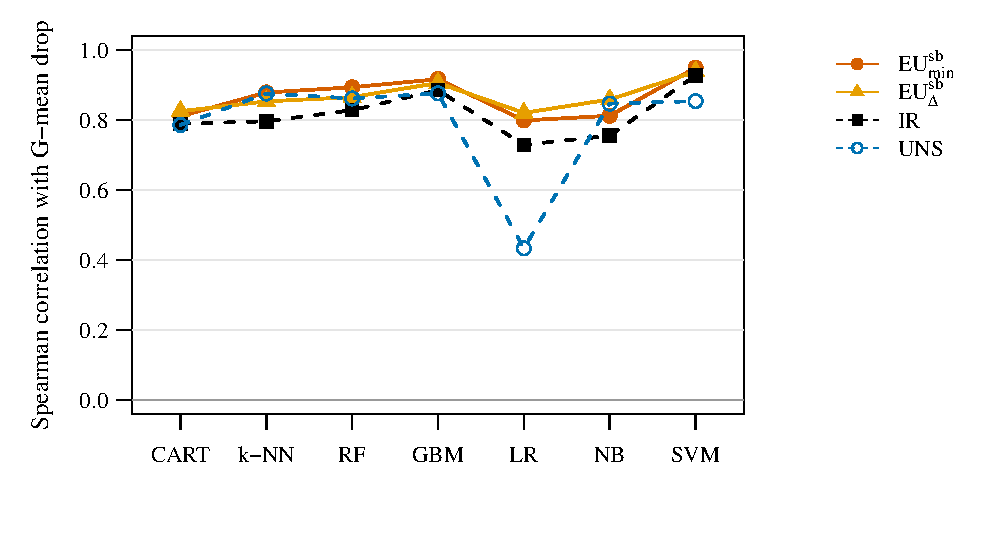
\includegraphics[width=0.85\textwidth]{figures/fig_sim_corr.pdf}
\caption{Simulation: Spearman correlation between the proposed measures and the two strongest competitors ($\IR$ and $\UNS$, by mean correlation) and the G-mean drop, by classifier (data of Table~\ref{tab:corr}).}\label{fig:simcorr}
\end{figure}

\begin{figure}[H]
\centering
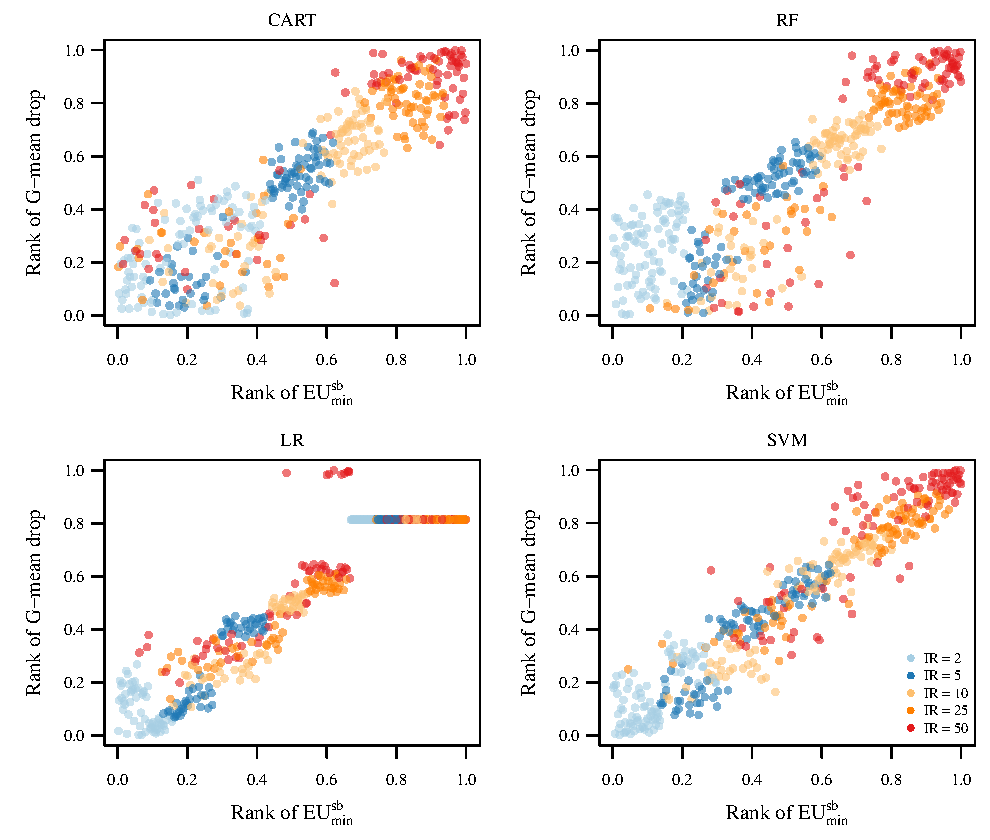
\includegraphics[width=0.85\textwidth]{figures/fig_sim_scatter.pdf}
\caption{Simulation: ranks of $\EUmin{sb}$ and of the G-mean drop for four classifiers ($\IR>1$; overlapping, disjunct and noise families). Colours show $\IR$. For LR the drop has many ties, because G-mean reaches zero when the minority is not predicted at all.}\label{fig:simscatter}
\end{figure}

Three readings follow. First, the ablation is clear: with plain votes ($\mathrm{EU}^{\mathrm{s}}$) or the hard split ($\mathrm{EU}^{\mathrm{h}}$) the correlation falls to 0.69 and 0.35 at best. Second, $\EUmin{sb}$ and $\EUdif{sb}$ stay between 0.80 and 0.95 for every classifier. Third, the classifier-independent measures collapse for logistic regression ($\UNS$ 0.43, $\RO$ 0.41, $\Nbal$ 0.25) while the proposed measures do not (0.80 and 0.82). This is the case for a classifier-aware measure. For the other classifiers $\UNS$ is close to the proposed measures, for example for $k$-NN (0.88 against 0.88 and 0.85) and RF (0.86 against 0.89 and 0.87).

\subsubsection{Added value over $\IR$}
We regress the cell-demeaned rank of the drop on $\IR$ as a factor and add one measure at a time. Table~\ref{tab:r2} gives the increase in $R^2$ over the model with $\IR$ alone ($R^2$ of $\IR$ alone: 0.65, 0.74, 0.56 and 0.88 for the four groups).

\begin{table}[H]
\centering
\caption{Increase in $R^2$ over the model with $\IR$ as a factor, by classifier group.}\label{tab:r2}
\begin{tabular}{lrrrr}
\toprule
Measure & Local & Ensemble & High-bias & Kernel \\
\midrule
$\EUmin{sb}$ & 0.131 & 0.102 & 0.222 & 0.055 \\
$\EUdif{sb}$ & 0.088 & 0.059 & 0.177 & 0.026 \\
$\EUmin{s}$ & 0.007 & 0.010 & 0.005 & 0.002 \\
$\EUdif{s}$ & 0.002 & 0.001 & 0.030 & 0.000 \\
$\EUdif{h}$ & 0.008 & 0.007 & 0.013 & 0.002 \\
$\UNS$ & 0.132 & 0.110 & 0.039 & 0.051 \\
$\Nbal$ & 0.152 & 0.099 & 0.047 & 0.057 \\
\bottomrule
\end{tabular}
\end{table}

$\EUmin{sb}$ adds information beyond $\IR$ in every group. In the local and ensemble groups it adds about as much as $\UNS$ and $\Nbal$. The gain is larger only in the high-bias group (0.222 against 0.039 for $\UNS$). With $\IR$ entered linearly instead of as a factor the additions roughly double ($\EUmin{sb}$ 0.24 to 0.33), so part of that larger figure is non-linearity in $\IR$, and we report the factor version. The plain-vote and hard-split variants add almost nothing.

\subsubsection{Separable data}
On the separable family the measures should be near zero. They are small but they grow with $\IR$, and the growth depends on the classifier (Table~\ref{tab:sep} and Fig.~\ref{fig:sep}).

\begin{table}[H]
\centering
\caption{Mean values of the measures on the separable family, by $\IR$ (all classifiers).}\label{tab:sep}
\small\setlength{\tabcolsep}{4pt}
\begin{tabular}{rrrrrrr}
\toprule
$\IR$ & $\EUmin{sb}$ & $\EUmin{s}$ & $\EUmin{h}$ & $\AUbal{sb}$ & $\AUbal{h}$ & $\AUbal{s}$ \\
\midrule
1 & 0.003 & 0.003 & 0.002 & 0.002 & 0.001 & 0.002 \\
10 & 0.011 & 0.013 & 0.008 & 0.002 & 0.003 & 0.005 \\
25 & 0.026 & 0.029 & 0.021 & 0.002 & 0.004 & 0.012 \\
50 & 0.048 & 0.057 & 0.040 & 0.001 & 0.007 & 0.021 \\
\bottomrule
\end{tabular}
\end{table}

\begin{figure}[H]
\centering
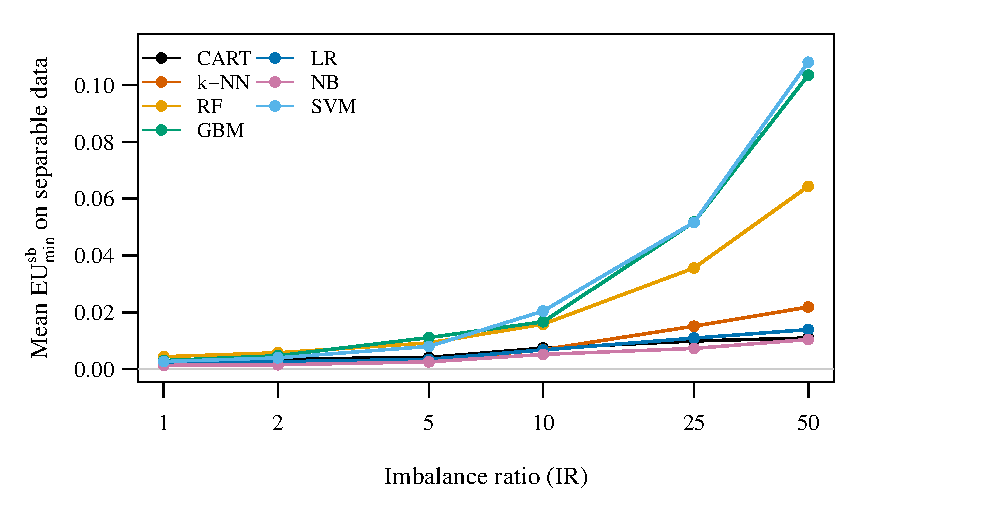
\includegraphics[width=0.85\textwidth]{figures/fig_sim_separable.pdf}
\caption{Simulation: mean $\EUmin{sb}$ on the separable family by $\IR$ and classifier.}\label{fig:sep}
\end{figure}

At $\IR=50$ the mean $\EUmin{sb}$ is 0.108 for SVM, 0.104 for GBM and 0.064 for RF, but only 0.010 to 0.022 for CART, NB, LR and $k$-NN. The Spearman correlation of $\EUmin{sb}$ with $\IR$ on separable data is 0.97 to 0.98 for RF, GBM and SVM, 0.68 for $k$-NN, 0.50 for NB, 0.37 for LR and 0.18 for CART. The balanced aleatoric variant $\AUbal{sb}$ stays flat.

\textbf{A reference level.} Among the 902 runs with ROC-AUC $=1$ on the test set, 95\% have $\EUmin{sb}\le 0.058$ and 99\% have $\EUmin{sb}\le 0.105$. A cut-off of 0.06 keeps 95\% of those runs and 2\% of the runs with ROC-AUC $<0.95$. The level depends on $\IR$: the 95th percentile is 0.004, 0.006, 0.009, 0.017, 0.048 and 0.094 for $\IR=1, 2, 5, 10, 25$ and 50. A single cut-off therefore works for $\IR$ up to about 10 and becomes loose at high $\IR$. For $\EUdif{sb}$, 0.06 keeps 97\% of the ROC-AUC $=1$ runs but also 29\% of the ROC-AUC $<0.95$ runs, so this reading applies to $\EUmin{sb}$ only.

\subsubsection{Aleatoric measures}
The aleatoric measures were compared with the same competitors on the noise side, with $\IR$ fixed. The best aleatoric variant, $\AUbal{sb}$, reaches a mean correlation of 0.83, against 0.85 for $\UNS$. They are therefore comparable with the existing measures but not better, which was the expected outcome, since they come as a by-product of the same computation.


\subsection{Real-data results}\label{sec:realres}
The simulation fixes the source of difficulty. The real-data study asks whether the measures predict where rebalancing helps on datasets whose difficulty is unknown.

\subsubsection{Gain from resampling}
Table~\ref{tab:real} gives the correlation with the gain in G-mean from SMOTE and from ROS, and Table~\ref{tab:other} the correlation with the gain from SMOTE in MCC and ROC-AUC (mean over the seven classifiers).

\begin{table}[H]
\centering
\caption{Spearman correlation between each measure and the gain in G-mean from resampling, across 30 datasets (mean over classifiers, bootstrap 95\% interval).}\label{tab:real}
\small\setlength{\tabcolsep}{4pt}
\begin{tabular}{lcc}
\toprule
Measure & SMOTE & ROS \\
\midrule
$\EUmin{sb}$ & 0.75 [0.64, 0.80] & 0.74 [0.63, 0.80] \\
$\EUdif{sb}$ & 0.70 [0.54, 0.80] & 0.68 [0.53, 0.77] \\
$\UNS$ & 0.64 [0.45, 0.76] & 0.60 [0.40, 0.72] \\
$\RO$ & 0.62 [0.45, 0.74] & 0.57 [0.37, 0.71] \\
$\Nbal$ & 0.53 [0.31, 0.69] & 0.50 [0.26, 0.64] \\
$\IR$ & 0.56 [0.36, 0.71] & 0.50 [0.28, 0.67] \\
$\EUdif{s}$ & 0.15 [$-0.15$, 0.38] & 0.16 [$-0.11$, 0.36] \\
$\EUmin{s}$ & $-0.03$ [$-0.33$, 0.25] & $-0.03$ [$-0.34$, 0.23] \\
$\EUdif{h}$ & 0.10 [$-0.21$, 0.40] & 0.16 [$-0.17$, 0.46] \\
$\EUmin{h}$ & $-0.01$ [$-0.33$, 0.34] & 0.04 [$-0.29$, 0.37] \\
\bottomrule
\end{tabular}
\end{table}

\begin{table}[H]
\centering
\caption{Spearman correlation between each measure and the SMOTE gain in MCC and in ROC-AUC, across 30 datasets (mean over classifiers, bootstrap 95\% interval).}\label{tab:other}
\small\setlength{\tabcolsep}{4pt}
\begin{tabular}{lcc}
\toprule
Measure & MCC gain & ROC-AUC gain \\
\midrule
$\EUmin{sb}$ & 0.40 [0.19, 0.54] & 0.31 [0.16, 0.45] \\
$\EUdif{sb}$ & 0.36 [0.17, 0.53] & 0.34 [0.18, 0.48] \\
$\UNS$ & 0.30 [0.10, 0.45] & 0.17 [$-0.02$, 0.39] \\
$\RO$ & 0.27 [0.08, 0.44] & 0.17 [$-0.02$, 0.39] \\
$\Nbal$ & 0.22 [0.01, 0.39] & 0.11 [$-0.07$, 0.31] \\
$\IR$ & 0.21 [0.01, 0.36] & 0.18 [0.01, 0.39] \\
$\EUdif{s}$ & $-0.07$ [$-0.29$, 0.11] & 0.07 [$-0.15$, 0.23] \\
$\EUdif{h}$ & $-0.07$ [$-0.28$, 0.17] & 0.02 [$-0.22$, 0.22] \\
\bottomrule
\end{tabular}
\end{table}

The pattern of the simulation repeats. The class-balanced soft measures lead, and the plain-vote and hard-split variants have intervals that contain zero. For MCC and ROC-AUC the correlations are lower for all measures, and the ordering is the same. The intervals of $\EUmin{sb}$ and of $\UNS$ and $\RO$ overlap, so with 30 datasets we do not claim that $\EUmin{sb}$ is better than these on the raw correlation alone. The distinction from $\mathrm{EU}^{\mathrm{s}}$ and $\mathrm{EU}^{\mathrm{h}}$ is clear, since their intervals lie below the lower limit of $\EUmin{sb}$.

\subsubsection{Results by classifier}
Table~\ref{tab:realclf} and Fig.~\ref{fig:realcorr} give the correlation with the SMOTE gain in G-mean for each classifier, and Fig.~\ref{fig:realscatter} shows the gain against $\EUmin{sb}$ for four classifiers.

\begin{table}[H]
\centering
\caption{Spearman correlation between each measure and the SMOTE gain in G-mean, by classifier (30 datasets).}\label{tab:realclf}
\small\setlength{\tabcolsep}{3pt}
\begin{tabular}{lrrrrrrrr}
\toprule
Measure & CART & $k$-NN & RF & GBM & LR & NB & SVM & Mean \\
\midrule
$\EUmin{sb}$ & 0.88 & 0.87 & 0.83 & 0.73 & 0.85 & 0.23 & 0.84 & 0.75 \\
$\EUdif{sb}$ & 0.79 & 0.78 & 0.72 & 0.69 & 0.76 & 0.55 & 0.63 & 0.70 \\
$\UNS$ & 0.71 & 0.73 & 0.69 & 0.66 & 0.74 & 0.17 & 0.78 & 0.64 \\
$\RO$ & 0.63 & 0.75 & 0.68 & 0.74 & 0.69 & 0.16 & 0.71 & 0.62 \\
$\Nbal$ & 0.55 & 0.62 & 0.57 & 0.62 & 0.64 & 0.04 & 0.68 & 0.53 \\
$\IR$ & 0.75 & 0.73 & 0.51 & 0.51 & 0.56 & 0.42 & 0.42 & 0.56 \\
\bottomrule
\end{tabular}
\end{table}

\begin{figure}[H]
\centering
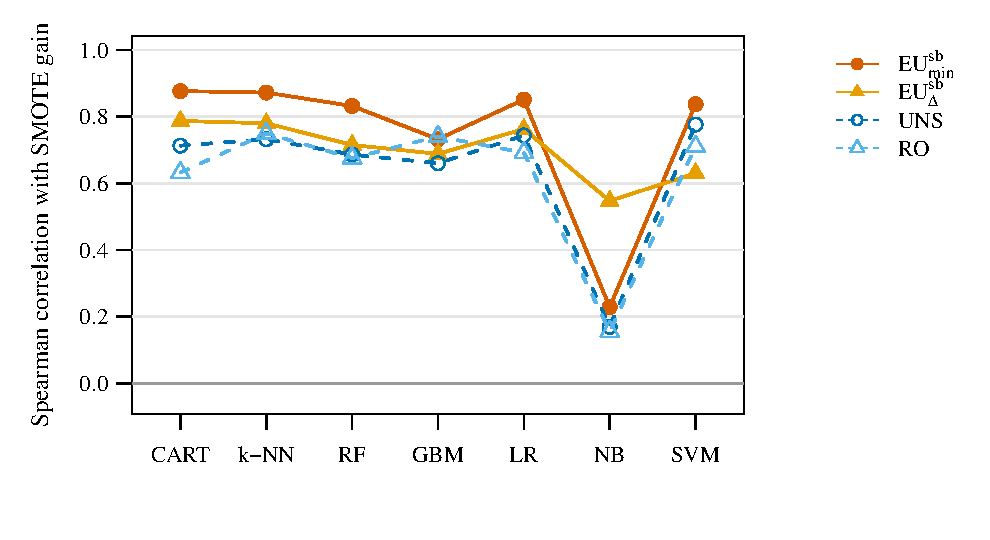
\includegraphics[width=0.85\textwidth]{figures/fig_real_corr.pdf}
\caption{Real data: Spearman correlation between the proposed measures and the two strongest competitors ($\UNS$ and $\RO$, by mean correlation) and the SMOTE gain in G-mean, by classifier (data of Table~\ref{tab:realclf}).}\label{fig:realcorr}
\end{figure}

\begin{figure}[H]
\centering
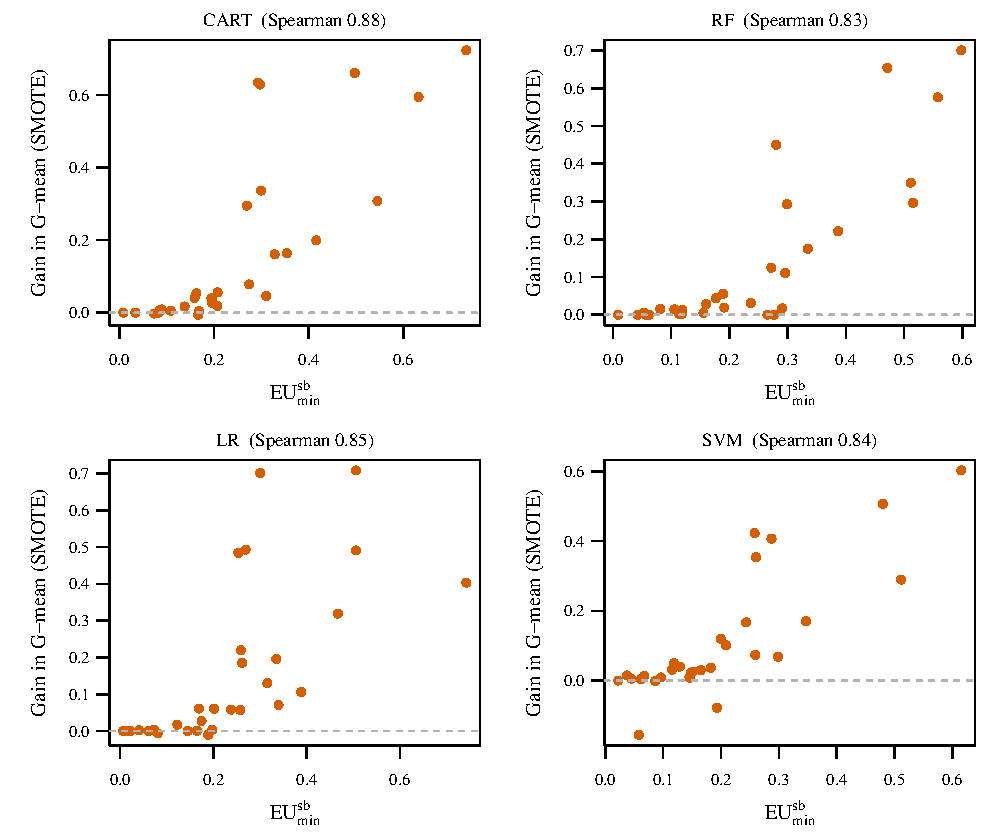
\includegraphics[width=0.85\textwidth]{figures/fig_real_scatter.pdf}
\caption{Real data: SMOTE gain in G-mean against $\EUmin{sb}$ for four classifiers, one point per dataset.}\label{fig:realscatter}
\end{figure}

For five of the seven classifiers (CART, $k$-NN, RF, LR and SVM) $\EUmin{sb}$ has the highest correlation of the measures in the table (0.83 to 0.88), and for GBM it is level with $\RO$ (0.73 against 0.74). Naive Bayes is the exception: the correlation of $\EUmin{sb}$ falls to 0.23, and the competitors fall as well ($\UNS$ 0.17, $\RO$ 0.16). The difference variant $\EUdif{sb}$ holds up better for NB (0.55) than the minimum variant, and $\IR$ is also higher there (0.42). We have not studied why NB behaves differently.

\subsubsection{Controlling for baseline performance}
Datasets that are already well classified cannot gain, so any measure that tracks difficulty correlates with gain. We therefore repeat the analysis with the rank of the NORES G-mean partialled out (Table~\ref{tab:partial}).

\begin{table}[H]
\centering
\caption{Partial Spearman correlation with the SMOTE gain in G-mean, controlling for the rank of the NORES G-mean (mean over classifiers, bootstrap 95\% interval).}\label{tab:partial}
\small\setlength{\tabcolsep}{4pt}
\begin{tabular}{lc}
\toprule
Measure & Partial Spearman \\
\midrule
$\EUdif{sb}$ & 0.58 [0.33, 0.71] \\
$\EUmin{sb}$ & 0.41 [0.20, 0.57] \\
$\IR$ & 0.39 [0.13, 0.56] \\
$\EUdif{s}$ & 0.36 [0.10, 0.55] \\
$\EUdif{h}$ & 0.28 [0.09, 0.45] \\
$\EUmin{s}$ & 0.03 [$-0.11$, 0.20] \\
$\EUmin{h}$ & $-0.01$ [$-0.17$, 0.17] \\
$\UNS$ & $-0.11$ [$-0.26$, 0.11] \\
$\RO$ & $-0.08$ [$-0.23$, 0.15] \\
$\Nbal$ & $-0.23$ [$-0.40$, 0.02] \\
\bottomrule
\end{tabular}
\end{table}

After control, $\EUdif{sb}$ has the highest partial correlation (0.58), and $\UNS$, $\RO$ and $\Nbal$ fall to about zero or below. Part of their raw correlation therefore comes from the baseline performance. $\EUmin{sb}$ (0.41) is not distinguishable from $\IR$ (0.39). The difference variants $\EUdif{s}$ (0.36) and $\EUdif{h}$ (0.28) keep a positive partial correlation, lower than that of $\EUdif{sb}$, while the minimum variants $\EUmin{s}$ and $\EUmin{h}$ stay at zero.


\subsection{A decision rule for oversampling}\label{sec:rule}
Table~\ref{tab:rule} gives the threshold of $\EUmin{sb}$ above which SMOTE pays off, for each metric, and Fig.~\ref{fig:threshold} shows the SMOTE gain against $\EUmin{sb}$.

\begin{table}[H]
\centering
\caption{Decision rule ``oversample if $\EUmin{sb}>\tau$'' (a SMOTE gain above $\delta=0.02$ counts as worth oversampling; 30 datasets, 7 classifiers, 210 pairs). Share: share of pairs worth oversampling. Sens., Spec., Bal. acc.: sensitivity, specificity and balanced accuracy in leave-one-dataset-out cross-validation (bootstrap 95\% interval in brackets). $\IR$ and $\UNS$: balanced accuracy of the same rule built on $\IR$ and on $\UNS$. Gain: mean gain when $\EUmin{sb}>\tau$ and when $\EUmin{sb}\le\tau$.}\label{tab:rule}
\scriptsize\setlength{\tabcolsep}{2pt}
\begin{tabular}{lrcrrcrrr}
\toprule
Metric & Share & $\tau$ & Sens. & Spec. & Bal. acc. & $\IR$ & $\UNS$ & Gain \\
\midrule
G-mean & 0.54 & 0.17 [0.14, 0.24] & 0.86 & 0.78 & 0.82 [0.75, 0.88] & 0.69 & 0.70 & 0.236 / 0.006 \\
MCC & 0.36 & 0.18 [0.18, 0.29] & 0.92 & 0.67 & 0.79 [0.72, 0.86] & 0.65 & 0.67 & 0.060 / $-$0.013 \\
ROC-AUC & 0.18 & 0.27 [0.26, 0.30] & 0.92 & 0.81 & 0.87 [0.81, 0.92] & 0.78 & 0.73 & 0.039 / $-$0.003 \\
P4 & 0.35 & 0.18 [0.18, 0.29] & 0.91 & 0.68 & 0.79 [0.72, 0.85] & 0.67 & 0.76 & 0.087 / $-$0.009 \\
\bottomrule
\end{tabular}
\end{table}

\begin{figure}[H]
\centering
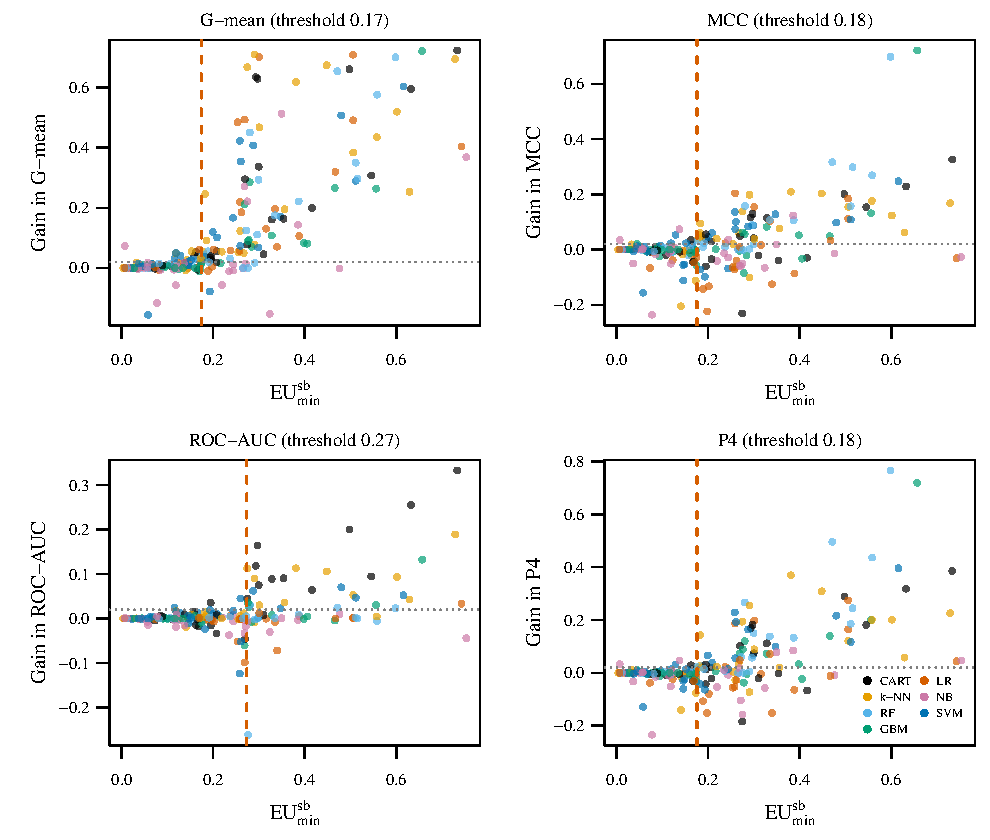
\includegraphics[width=0.85\textwidth]{figures/fig_real_threshold.pdf}
\caption{Real data: SMOTE gain against $\EUmin{sb}$ for four metrics, one point per classifier and dataset. The dashed vertical line is the threshold $\tau$ of Table~\ref{tab:rule} and the dotted horizontal line is $\delta=0.02$.}\label{fig:threshold}
\end{figure}

\begin{figure}[H]
\centering
(a) Epistemic measure $\EUmin{sb}$\\[2pt]
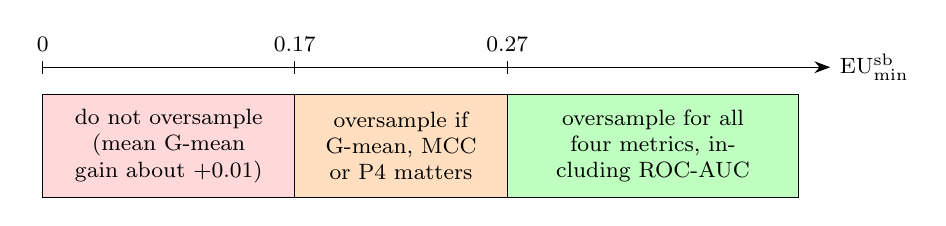
\begin{tikzpicture}[font=\footnotesize, >={Stealth[length=2mm]}]
\def\y{0}
\fill[red!15] (0,\y) rectangle (3.2,\y-1.3);
\fill[orange!25] (3.2,\y) rectangle (5.9,\y-1.3);
\fill[green!25] (5.9,\y) rectangle (9.6,\y-1.3);
\draw (0,\y) rectangle (9.6,\y-1.3);
\draw (3.2,\y)--(3.2,\y-1.3);
\draw (5.9,\y)--(5.9,\y-1.3);
\node[align=center, text width=3.00cm] at (1.6,\y-0.65) {do not oversample\\ (mean G-mean gain about $+0.01$)};
\node[align=center, text width=2.50cm] at (4.550000000000001,\y-0.65) {oversample if G-mean, MCC or P4 matters};
\node[align=center, text width=3.50cm] at (7.75,\y-0.65) {oversample for all four metrics, including ROC-AUC};
\draw[->] (0,\y+0.35)--(10.0,\y+0.35) node[right] {$\EUmin{sb}$};
\foreach \x/\l in {0/0,3.2/0.17,5.9/0.27}{\draw (\x,\y+0.27)--(\x,\y+0.43) node[above] {\l};}
\end{tikzpicture}
\\[10pt]
(b) Epistemic difference measure $\EUdif{sb}$\\[2pt]
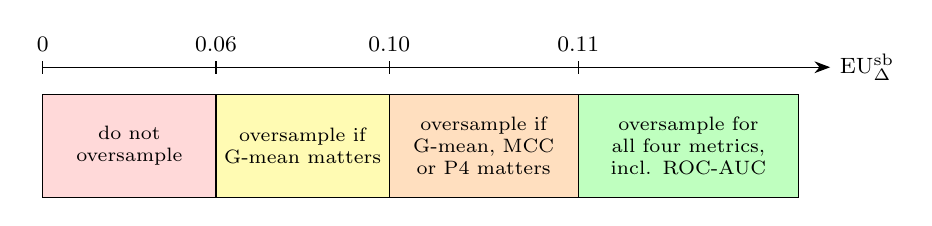
\begin{tikzpicture}[font=\footnotesize, >={Stealth[length=2mm]}]
\def\y{0}
\fill[red!15] (0,\y) rectangle (2.2,\y-1.3);
\fill[yellow!30] (2.2,\y) rectangle (4.4,\y-1.3);
\fill[orange!25] (4.4,\y) rectangle (6.8,\y-1.3);
\fill[green!25] (6.8,\y) rectangle (9.6,\y-1.3);
\draw (0,\y) rectangle (9.6,\y-1.3);
\draw (2.2,\y)--(2.2,\y-1.3);
\draw (4.4,\y)--(4.4,\y-1.3);
\draw (6.8,\y)--(6.8,\y-1.3);
\node[align=center, font=\scriptsize, text width=2.00cm] at (1.1,\y-0.65) {do not oversample};
\node[align=center, font=\scriptsize, text width=2.00cm] at (3.3000000000000003,\y-0.65) {oversample if G-mean matters};
\node[align=center, font=\scriptsize, text width=2.20cm] at (5.6,\y-0.65) {oversample if G-mean, MCC or P4 matters};
\node[align=center, font=\scriptsize, text width=2.60cm] at (8.2,\y-0.65) {oversample for all four metrics, incl. ROC-AUC};
\draw[->] (0,\y+0.35)--(10.0,\y+0.35) node[right] {$\EUdif{sb}$};
\foreach \x/\l in {0/0,2.2/0.06,4.4/0.10,6.8/0.11}{\draw (\x,\y+0.27)--(\x,\y+0.43) node[above] {\l};}
\end{tikzpicture}
\caption{Guide for deciding whether to oversample, using the measure computed on the training data with the chosen classifier. (a) Thresholds 0.17 for the G-mean, 0.18 for MCC and P4, and 0.27 for ROC-AUC (Table~\ref{tab:rule}). (b) Thresholds 0.06 for the G-mean, 0.10 for MCC and P4, and 0.11 for ROC-AUC. Zone widths are not to scale and the guide is preliminary.}\label{fig:guide}
\end{figure}

For the G-mean the threshold is 0.17. Above it, SMOTE raised the G-mean by 0.24 on average; at or below it, by 0.01. In cross-validation the rule classified the pairs with a balanced accuracy of 0.82, against 0.69 for the rule built on $\IR$ and 0.70 for $\UNS$. The thresholds for MCC and P4 are also 0.18, with balanced accuracies of 0.79 against 0.65 to 0.67 for $\IR$. The ROC-AUC threshold is higher (0.27), because ROC-AUC changes less with resampling and only 18\% of the pairs gain more than 0.02. The bootstrap interval of $\tau$ is wide for the G-mean (0.14 to 0.24) and narrower for the other metrics. For each classifier separately, $\EUmin{sb}$ separates the pairs worth oversampling from the others with an area under the ROC curve of 0.92 to 1.00 for the G-mean for six classifiers and 0.79 for naive Bayes (0.55 for MCC). The difference variant $\EUdif{sb}$ (Fig.~\ref{fig:guide}b) gives thresholds of 0.06 for the G-mean, 0.10 for MCC and P4, and 0.11 for ROC-AUC. Its balanced accuracy in cross-validation equals that of $\EUmin{sb}$ for the G-mean (0.83) and is lower for the other metrics (0.72 to 0.76). The results are similar for $\delta=0.01$ and $\delta=0.05$ (threshold 0.17 to 0.20, balanced accuracy 0.82 to 0.88 for SMOTE) and for random oversampling (0.79 to 0.85).

\begin{figure}[H]
\centering
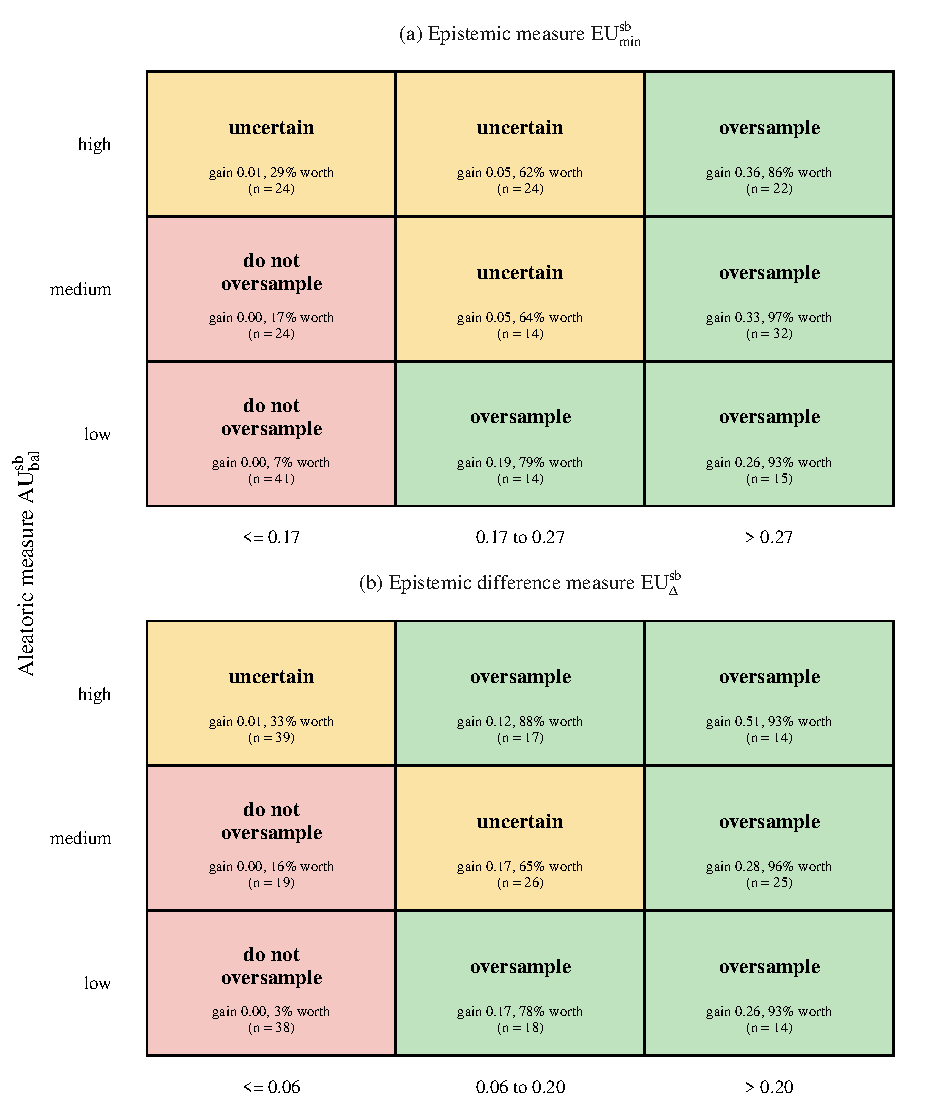
\includegraphics[width=0.68\textwidth]{figures/fig_real_heatmap.pdf}
\caption{Exploratory guide with both uncertainty parts, for combinations of (a) $\EUmin{sb}$ (bands at 0.17 and 0.27) or (b) $\EUdif{sb}$ (bands at 0.06 and 0.20) and $\AUbal{sb}$ (terciles, cut at 0.045 and 0.095). Each cell gives the mean SMOTE gain in G-mean, the share of classifier--dataset pairs whose gain exceeds 0.02 (``worth'') and the number of pairs. A cell is marked ``do not oversample'' if fewer than 25\% of its pairs are worth it, ``oversample'' if more than 75\% are, and ``uncertain'' otherwise}\label{fig:heatmap}
\end{figure}

Fig.~\ref{fig:heatmap} adds the aleatoric measure. Below $\EUmin{sb}=0.17$ the gain is near zero whatever the aleatoric level, and above 0.27 it is large (0.26 to 0.36). The aleatoric measure matters in the middle band: the mean gain is 0.19 when $\AUbal{sb}$ is low and 0.05 when it is medium or high, which agrees with the idea that oversampling helps less when the errors come from noise and overlap. Alone, $\AUbal{sb}$ is unrelated to the gain (Spearman 0.07), and in the top band the gain does not fall with $\AUbal{sb}$, probably because the two measures rise together (Spearman 0.24). For $\EUdif{sb}$ (Fig.~\ref{fig:heatmap}b) the picture is similar in the extremes (no gain below 0.06 for medium and low $\AUbal{sb}$, gain above 0.20 in all cells), but the aleatoric measure does not help in the middle band: pairs with high $\AUbal{sb}$ gain as often as those with low $\AUbal{sb}$ (88\% against 78\%). Here the two measures are negatively related (Spearman $-0.20$), unlike for $\EUmin{sb}$. The cells hold 14 to 41 pairs, and the seven classifiers share the same datasets, so we treat Fig.~\ref{fig:heatmap} as exploratory.

%% =====================================================================
\section{Discussion and limitations}\label{sec:disc}
\textbf{What the measure captures.} The class-balanced neighbour vote is what makes the epistemic measure work. It equals the plain-vote odds multiplied by $n_0/n_1$, a logit shift of $\log(n_0/n_1)$ on the neighbour side only, while the model probability stays raw. We therefore read $\mathrm{EU}^{\mathrm{sb}}$ as the disagreement between a raw model and a balanced local posterior. That disagreement includes the prior shift that resampling removes, which fits the real-data result. We have not separated the prior-shift part from the rest, for example with a symmetric variant, and we leave it open.

\textbf{Limitations.}
\begin{itemize}
\item Growth with $\IR$ on separable data: the epistemic measures are small but rise with $\IR$ ($\EUmin{sb}$ 0.003 to 0.048 on average, and to about 0.10 for SVM and GBM at $\IR=50$), so they are not zero for separable data at high imbalance. The ROC-AUC $=1$ reference level of about 0.06 holds only for $\IR$ up to about 10.
\item $\EUmin{sb}$ is not separated from $\IR$ once baseline performance is controlled (0.41 against 0.39); $\EUdif{sb}$ is (0.58). Among the plain-vote and hard-split variants only the difference versions keep a positive partial correlation (0.36 and 0.28).
\item Added value over $\IR$ is about as large as that of $\UNS$ and $\Nbal$ for local and ensemble classifiers. The clear gain is for the high-bias and, partly, the kernel classifiers.
\item Naive Bayes behaves differently on real data (correlation 0.23 for $\EUmin{sb}$), and we have no explanation yet.
\item LR and NB lose G-mean mainly through the decision threshold, not through ranking, so ROC-AUC barely drops and is uninformative for them. We therefore use G-mean as the main metric.
\item The aleatoric measures are weak: $\AUbal{sb}$ reaches 0.83 against 0.85 for $\UNS$, and on real data they were used only in an exploratory grid (Fig.~\ref{fig:heatmap}).
\item The decision rule is preliminary. It was derived on 30 datasets and checked only by leave-one-dataset-out cross-validation, so it needs independent datasets. It depends on how the measure is computed (15 neighbours, 30 ensemble members, scaled features), was built for SMOTE and random oversampling with a gain threshold $\delta=0.02$, and is less reliable for naive Bayes.
\item The real datasets are binary, tabular, with 6 to 20 features and 200 to 2\,900 cases. The threshold was less accurate for the datasets with more than 10 features (0.76 against 0.87 to 0.88), so datasets of other types may need a new calibration.
\item Only the case where the minority class is the smaller one ($\IR>1$) was tested, and the real-data study has 30 datasets.
\item The overlap measures (N1 to N4, LSC) correlate with the imbalance-driven drop with the wrong sign, because they were designed for overlap and not for imbalance.
\end{itemize}

%% =====================================================================
\section{Conclusion}\label{sec:concl}
We proposed an epistemic-uncertainty complexity measure for class imbalance that depends on the classifier, built from out-of-bag predictions of bootstrap ensembles and compared with a class-balanced neighbour posterior. In simulation it follows the G-mean lost to imbalance with a Spearman correlation of about 0.87 to 0.89, stays between 0.80 and 0.95 for every classifier, and adds information beyond the imbalance ratio. On 30 real datasets it correlates with the gain from resampling (0.75, and 0.58 after controlling for baseline performance for $\EUdif{sb}$), where the plain-vote and hard-split variants do not, with naive Bayes as the exception. Its limits are a rise with $\IR$ on separable data and a weaker advantage over simple neighbourhood measures for local and ensemble classifiers. From the real-data results we derived a preliminary guide: compute $\EUmin{sb}$ on the training data with the classifier to be used, and oversample if it exceeds about 0.17 for G-mean, MCC and P4, or about 0.27 for ROC-AUC, and a grid that adds the aleatoric measure for the cases near the threshold. In cross-validation this rule classified 79\% to 87\% of the classifier--dataset pairs correctly, against 65\% to 78\% for the rule built on $\IR$. Future work includes validating the guide on independent datasets, a design for aleatoric measures on real data, the $\IR<1$ direction and a test of the prior-shift reading.

%% =====================================================================
\section*{CRediT authorship contribution statement}
\textbf{Fatih Sa\u{g}lam:} Conceptualization, Methodology, Software, Formal analysis, Investigation, Visualization, Writing -- original draft, Writing -- review and editing.

\section*{Declaration of competing interest}
The author declares that he has no known competing financial interests or personal relationships that could have appeared to influence the work reported in this paper.

\section*{Funding}
This research did not receive any specific grant from funding agencies in the public, commercial, or not-for-profit sectors.

\section*{Data availability}
The 30 real datasets are publicly available from the UCI Machine Learning Repository~\cite{UCI} and the KEEL dataset repository~\cite{Alcala2011}, and the sources are cited in the text. The simulated data are generated by the procedure described in Section~\ref{sec:simdesign}. The code and the results of the simulation and of the real-data study are available from the author on request.

\section*{Declaration of generative AI and AI-assisted technologies in the manuscript preparation process}
During the preparation of this work the author used Claude (Anthropic) to assist with writing and running analysis code and with drafting and editing the manuscript text. After using this tool, the author reviewed and edited the content as needed and takes full responsibility for the content of the published article.

\bibliographystyle{elsarticle-num}
\bibliography{refs}

\end{document}
